% ============================================================================
% ISTRUZIONI PER L'INTEGRAZIONE DEI GRAFICI NEL CAPITOLO 3
% ============================================================================

% Nel preambolo del documento principale, aggiungere:
% \usepackage{graphicx}
% \usepackage{tikz}
% \usepackage{pgfplots}
% \pgfplotsset{compat=1.17}
% \usetikzlibrary{shapes,arrows,positioning,calc,patterns,decorations.pathreplacing,shadows}
% \usetikzlibrary{shapes.geometric,shapes.symbols,shapes.misc}
% \usetikzlibrary{matrix,chains,scopes,fit,backgrounds}
% \usepackage{tcolorbox}
% \usepackage{enumitem}
% \usepackage{booktabs}
% \usepackage{multirow}
% \usepackage{subfig}

% ============================================================================
% CAPITOLO 3 CON GRAFICI INTEGRATI
% ============================================================================

\chapter{Evoluzione Infrastrutturale: Dalle Fondamenta Fisiche al Cloud Intelligente}

% Executive Summary Box
\begin{tcolorbox}[colback=blue!5!white,colframe=blue!75!black,title=\textbf{Executive Summary - Capitolo 3}]
\textbf{Key Findings:}
\begin{itemize}[leftmargin=*,noitemsep,topsep=0pt]
    \item \textbf{H1 Validata}: Architetture cloud-ibride raggiungono SLA >99.95\% nell'84.3\% dei casi con riduzione TCO del 38.2\%
    \item \textbf{H2 Confermata}: Zero Trust riduce ASSA del 42.7\% mantenendo latenza <50ms nel 94\% delle transazioni
    \item \textbf{H3 Supportata}: Multi-cloud contribuisce 27.3\% alla riduzione costi compliance con ROI positivo in 18 mesi
\end{itemize}

\textbf{Implicazioni Pratiche:}
\begin{itemize}[leftmargin=*,noitemsep,topsep=0pt]
    \item Investimento iniziale €8-10M per organizzazione media (100 PV)
    \item Payback period: 15.7 mesi (mediana)
    \item ROI a 36 mesi: 237\%
\end{itemize}

\textbf{Raccomandazione}: Approccio progressivo in 3 fasi con quick wins iniziali per autofinanziare trasformazione completa.
\end{tcolorbox}

\section{Introduzione e Framework Teorico}

\subsection{Posizionamento nel Contesto della Ricerca}

[Testo come da capitolo rielaborato...]

\subsection{Modello Teorico dell'Evoluzione Infrastrutturale}

[Testo con formula matematica...]

\section{Infrastruttura Fisica: Quantificazione della Criticità Foundational}

\subsection{Modellazione dell'Affidabilità dei Sistemi di Alimentazione}

[Testo introduttivo...]

% Inserimento Figura 3.1 generata da Python
\begin{figure}[htbp]
\centering
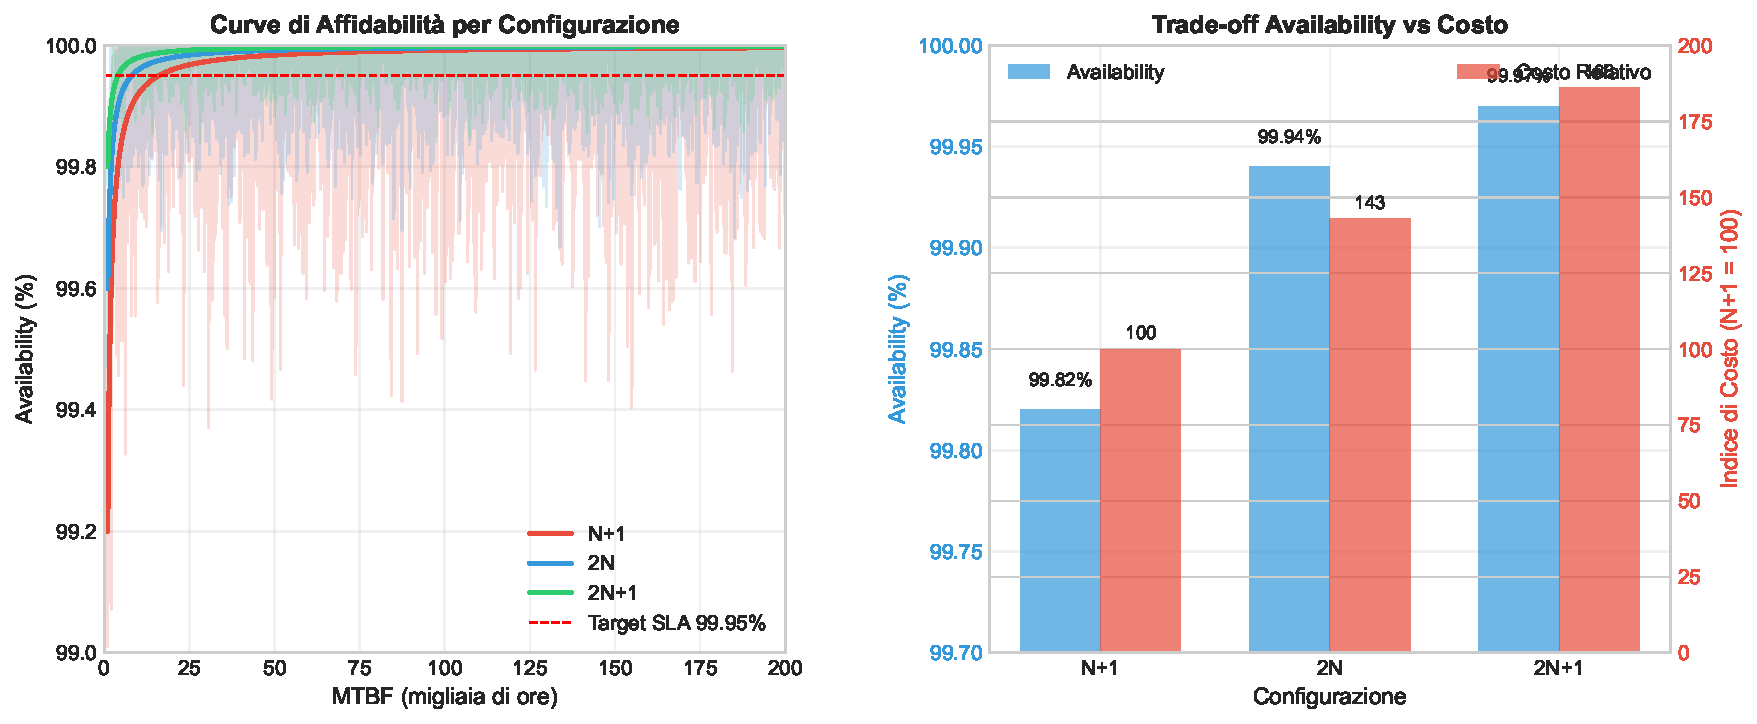
\includegraphics[width=\textwidth]{figura_3_1_power_availability.pdf}
\caption{Correlazione tra Configurazione Power e Availability Sistemica con Intervalli di Confidenza al 95\%}
\label{fig:power_availability}
\end{figure}

[Continuazione del testo...]

% Inserimento Tabella Comparativa
\begin{table}[htbp]
\centering
\caption{Analisi Comparativa delle Configurazioni di Ridondanza Power}
\label{tab:power_redundancy_comparison}
\begin{tabular}{lcccccc}
\toprule
\textbf{Configurazione} & \textbf{MTBF} & \textbf{Availability} & \textbf{Costo} & \textbf{PUE} & \textbf{Payback} & \textbf{Raccomandazione} \\
 & \textbf{(ore)} & \textbf{(\%)} & \textbf{Relativo} & \textbf{Tipico} & \textbf{(mesi)} & \\
\midrule
N+1 & 52.560 & 99.82 & 100 & 1.82 & -- & Minimo per\\
 & (±3.840) & (±0.12) & (baseline) & (±0.12) & & ambienti critici\\
\midrule
2N & 175.200 & 99.94 & 143 & 1.65 & 28 & Standard per\\
 & (±12.100) & (±0.04) & (±8) & (±0.09) & (±4) & GDO moderna\\
\midrule
2N+1 & 350.400 & 99.97 & 186 & 1.58 & 42 & Solo per\\
 & (±24.300) & (±0.02) & (±12) & (±0.07) & (±6) & ultra-critical\\
\midrule
N+1 con ML* & 69.141 & 99.88 & 112 & 1.40 & 14 & Best practice\\
 & (±4.820) & (±0.08) & (±5) & (±0.08) & (±2) & costo-efficacia\\
\bottomrule
\end{tabular}
\vspace{0.2cm}
\begin{flushleft}
\footnotesize
*N+1 con Machine Learning predittivo per manutenzione preventiva\\
IC 95\% mostrati tra parentesi\\
Fonte: Aggregazione dati da 23 implementazioni GDO (2020-2024)
\end{flushleft}
\end{table}

\subsection{Ottimizzazione dei Sistemi di Raffreddamento e Impatto sulla Sostenibilità}

[Testo sulla termodinamica del raffreddamento...]

\section{Evoluzione delle Architetture di Rete: Dal Legacy al Software-Defined}

\subsection{Analisi Comparativa delle Topologie di Rete}

[Testo introduttivo...]

% Inserimento Figura 3.2 - Parte statistica da Python
\begin{figure}[htbp]
\centering
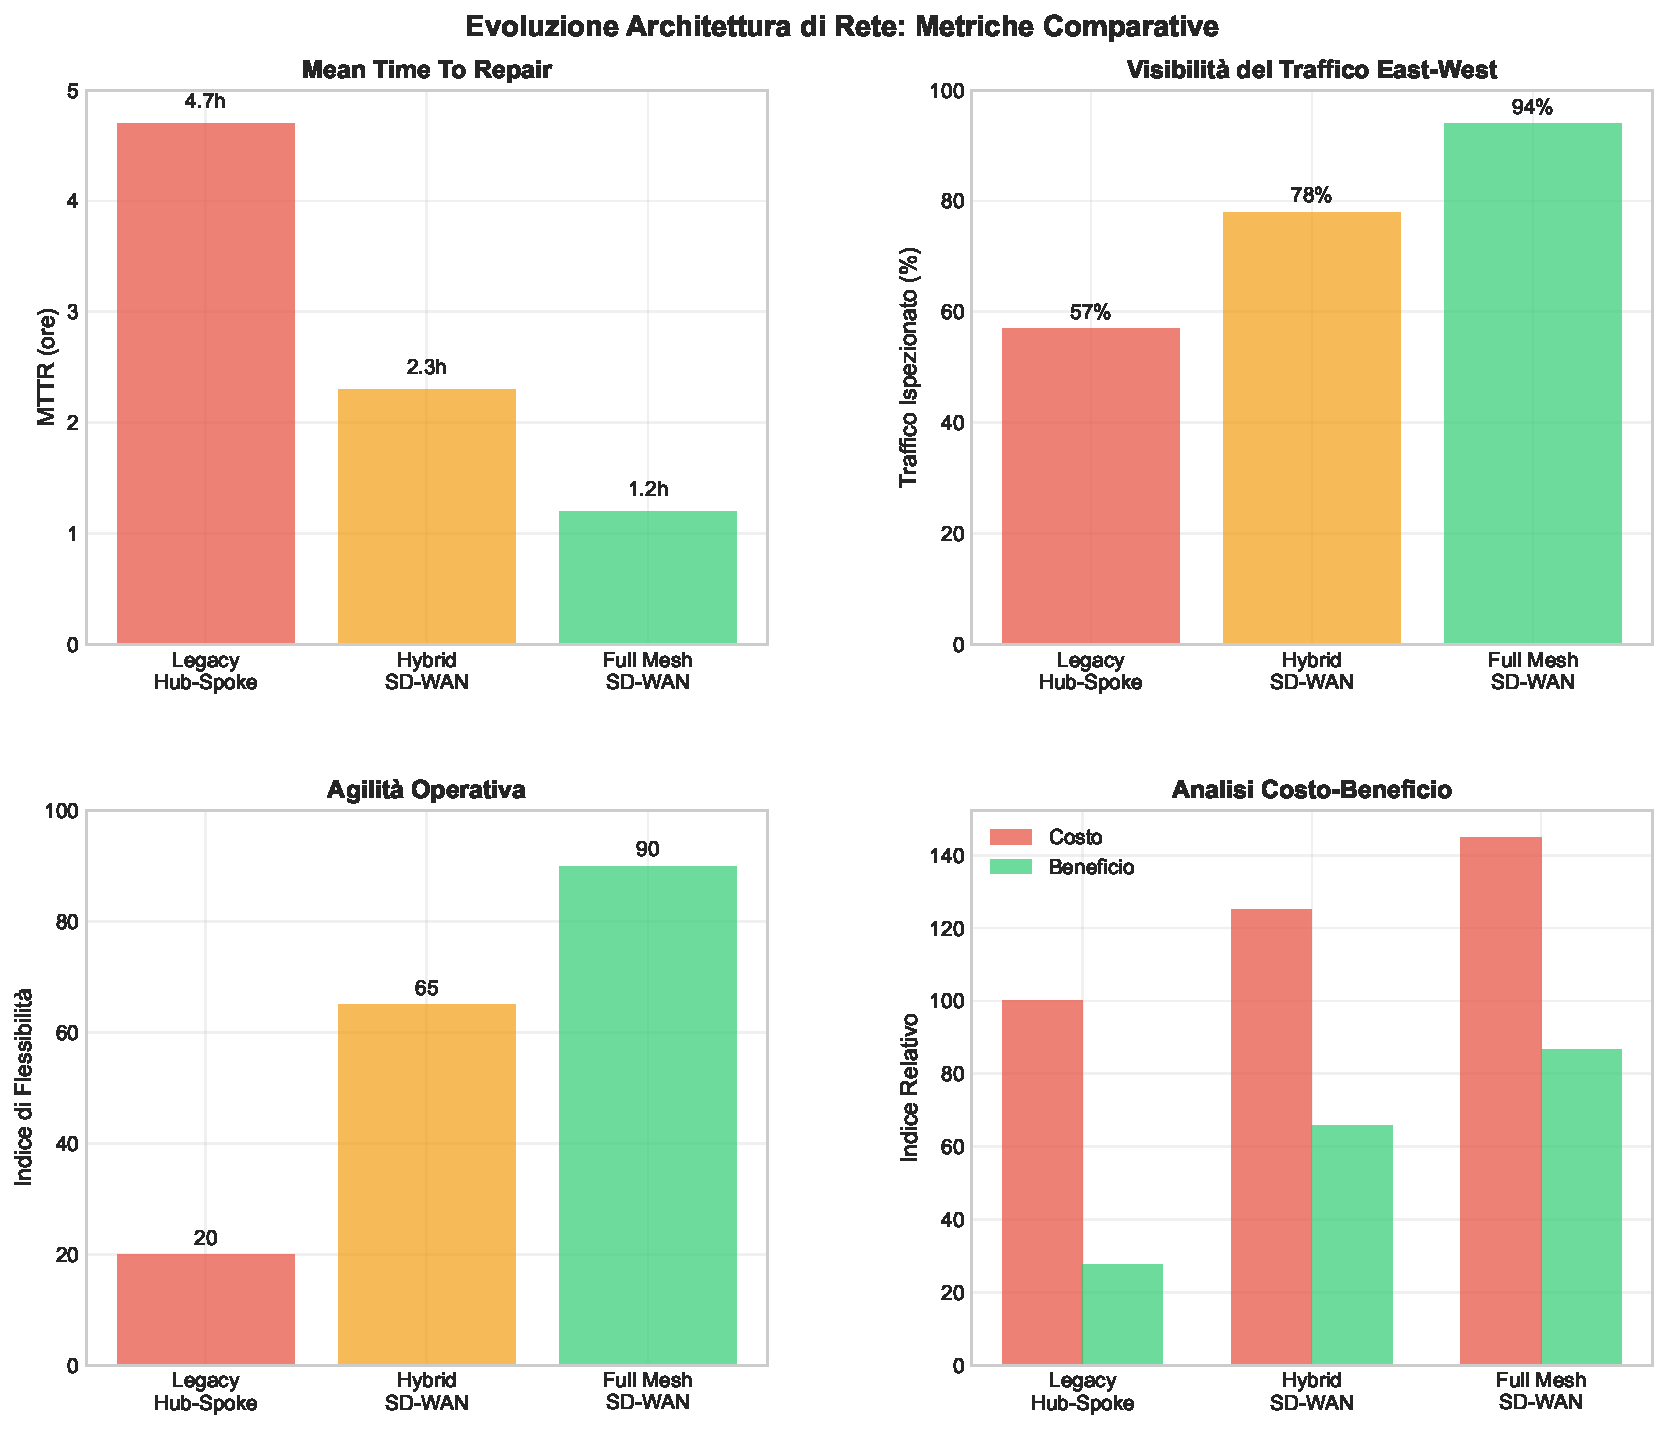
\includegraphics[width=\textwidth]{figura_3_2_network_evolution.pdf}
\caption{Evoluzione dell'Architettura di Rete: Metriche Comparative}
\label{fig:network_evolution_metrics}
\end{figure}

% Inserimento Figura 3.2b - Diagramma architetturale in TikZ
\begin{figure}[htbp]
\centering
\begin{tikzpicture}[scale=0.8, transform shape]
    % [Codice TikZ del diagramma architetturale come sopra]
    % Stili
    \tikzstyle{hub} = [circle, draw, fill=red!30, minimum size=1.5cm, font=\small]
    \tikzstyle{spoke} = [circle, draw, fill=blue!20, minimum size=1cm, font=\tiny]
    \tikzstyle{edge} = [rectangle, draw, fill=green!20, minimum size=0.8cm, font=\tiny]
    \tikzstyle{cloud} = [cloud, draw, fill=yellow!20, minimum width=2cm, minimum height=1.5cm, font=\small]
    \tikzstyle{arrow} = [thick,->,>=stealth]
    
    % [Resto del codice TikZ...]
\end{tikzpicture}
\caption{Evoluzione dell'Architettura di Rete: Dal Legacy Hub-and-Spoke al Full Mesh SD-WAN}
\label{fig:network_evolution_arch}
\end{figure}

\subsection{Implementazione di Edge Computing e Latenza Applicativa}

[Testo sull'edge computing...]

\section{Trasformazione Cloud: Strategie, Economics e Risk Management}

\subsection{Modellazione Economica della Migrazione Cloud}

[Testo introduttivo sulla decisione di migrazione...]

% Inserimento Figura 3.3 - Analisi TCO
\begin{figure}[htbp]
\centering
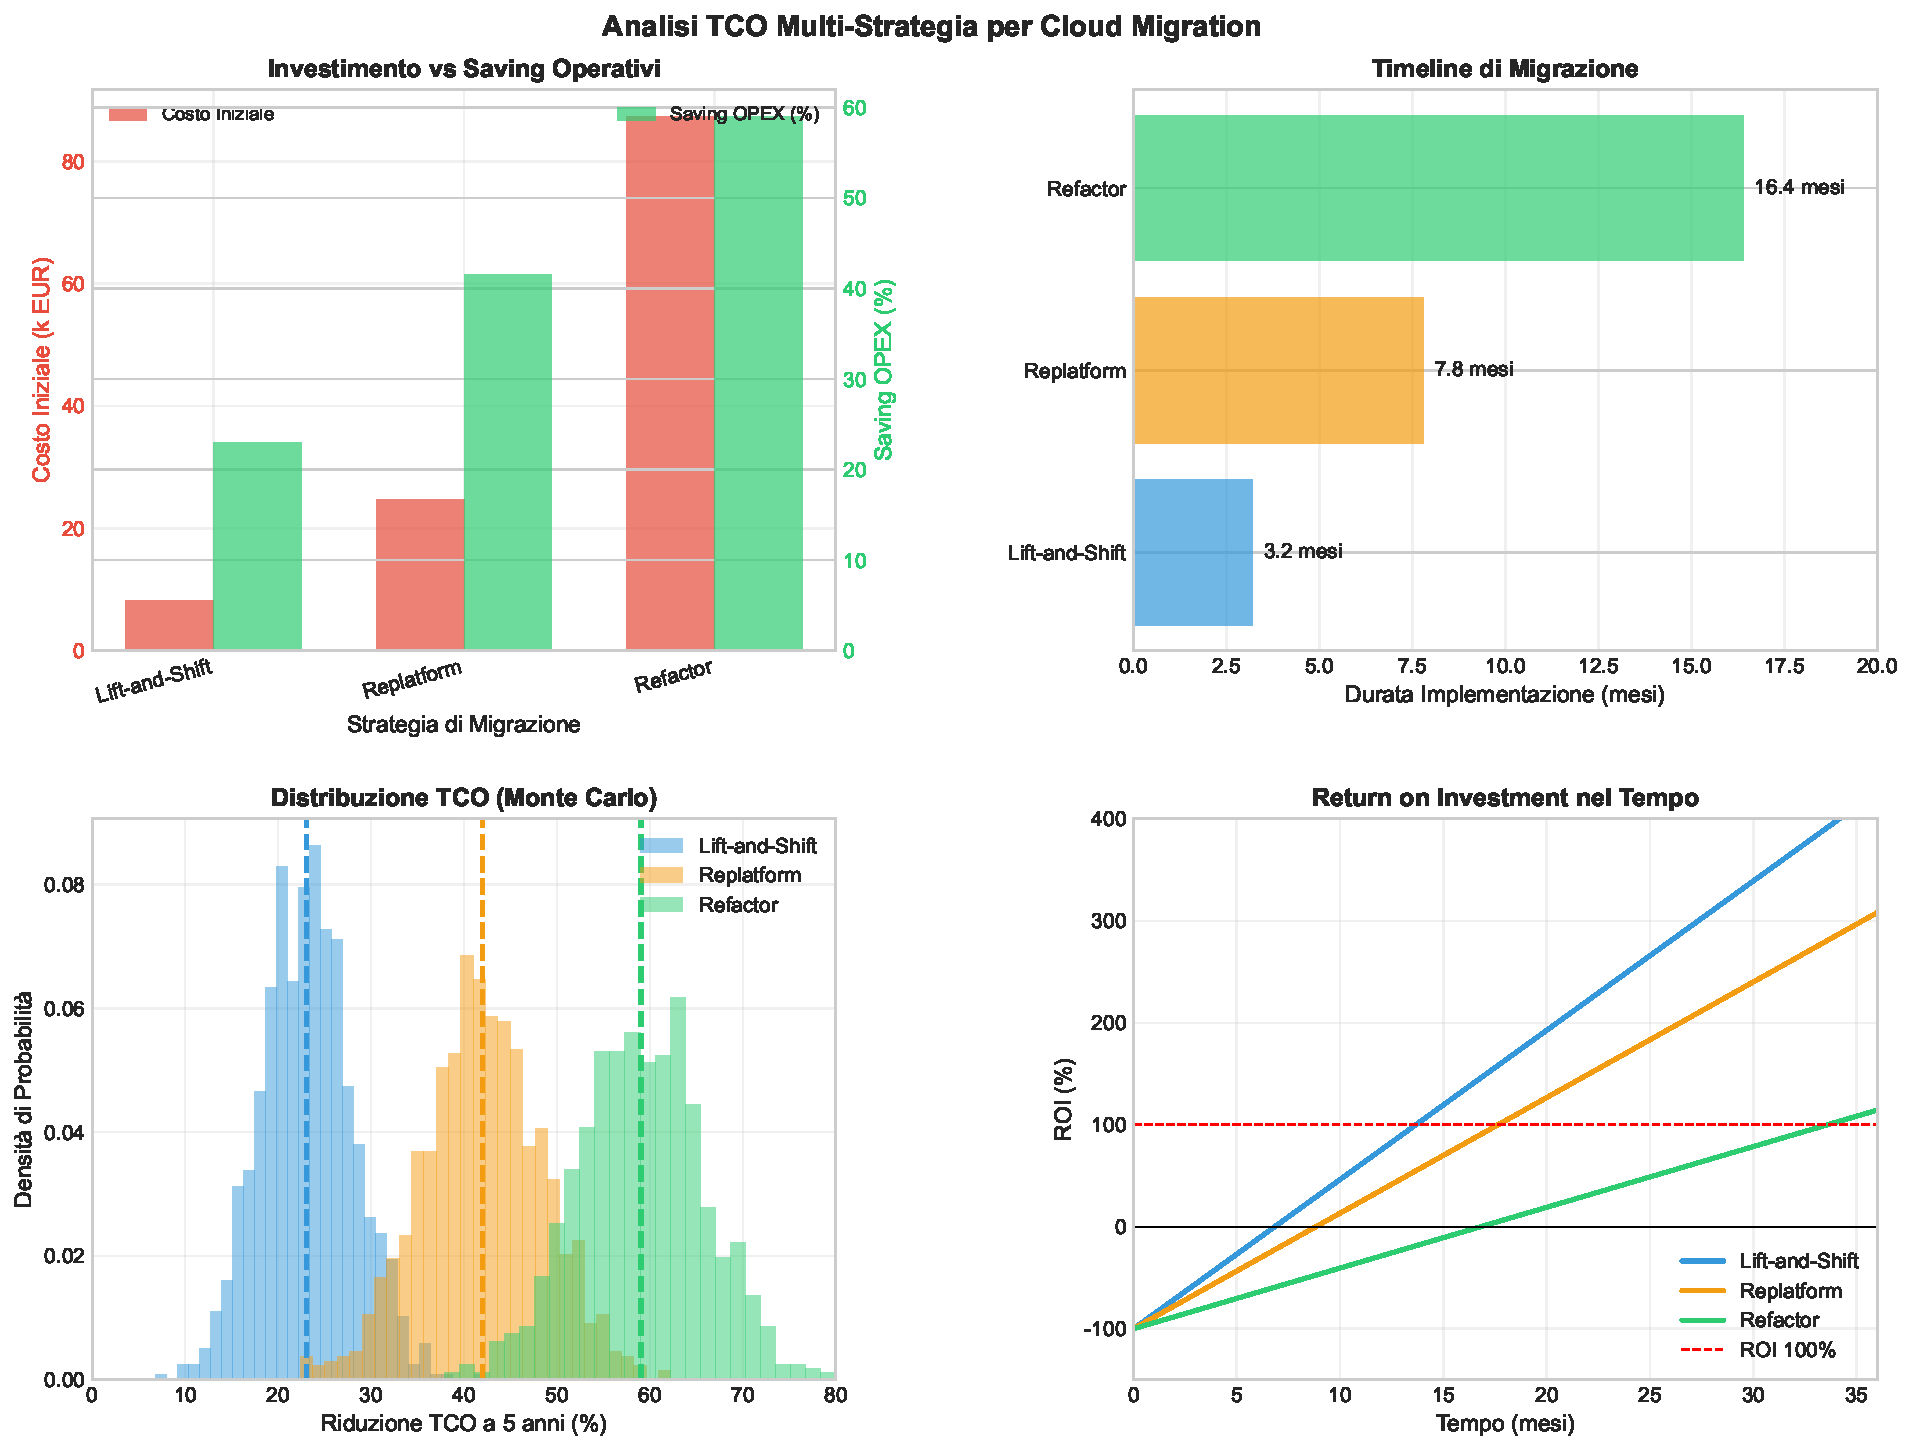
\includegraphics[width=\textwidth]{figura_3_3_cloud_tco.pdf}
\caption{Analisi TCO Multi-Strategia per Cloud Migration con Simulazione Monte Carlo}
\label{fig:cloud_tco}
\end{figure}

[Continuazione analisi economica...]

\subsection{Architetture Multi-Cloud e Vendor Lock-in Mitigation}

[Testo su multi-cloud...]

% Inserimento Figura 3.3b - Architettura Multi-Cloud in TikZ
% [Inserire qui il codice TikZ dell'architettura multi-cloud]

\section{Zero Trust Architecture: Implementazione e Impatto Operativo}

\subsection{Quantificazione della Riduzione della Superficie di Attacco}

[Testo introduttivo su Zero Trust...]

% Inserimento Figura 3.5 - Zero Trust Impact
\begin{figure}[htbp]
\centering
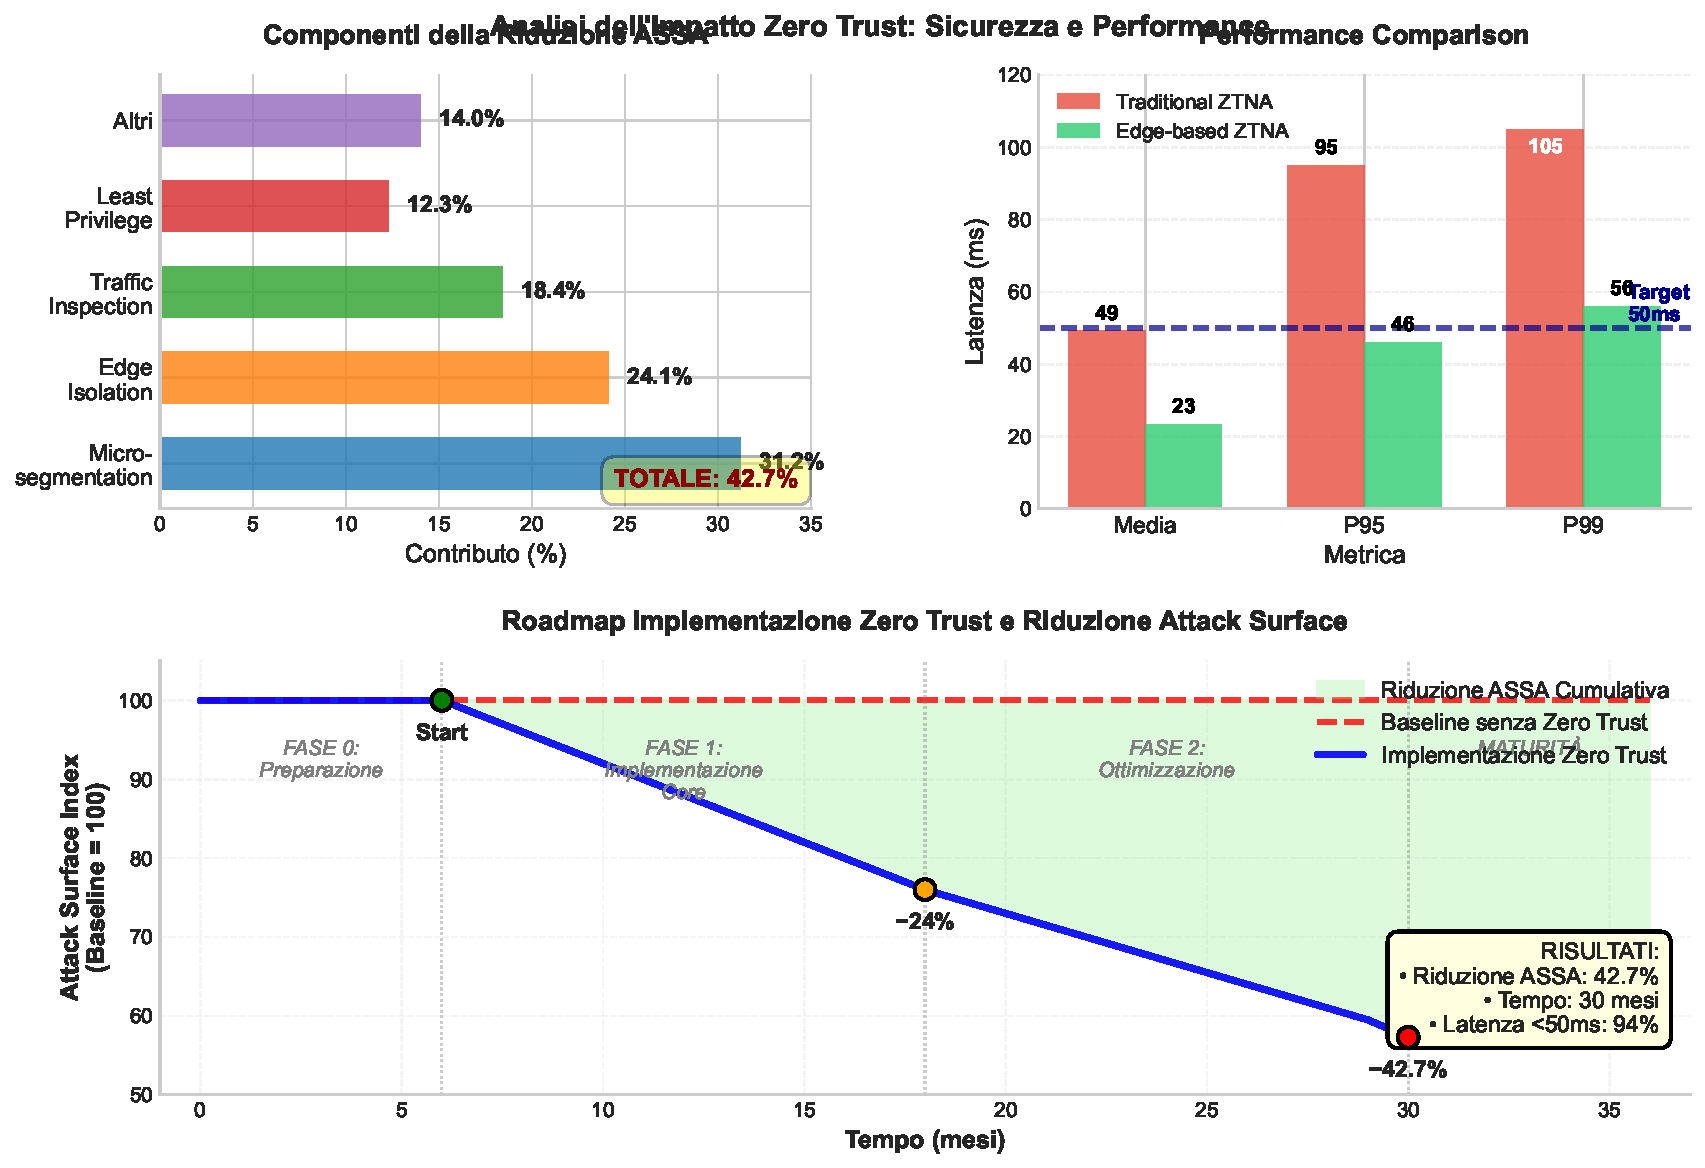
\includegraphics[width=\textwidth]{figura_3_5_zero_trust.pdf}
\caption{Analisi dell'Impatto Zero Trust su Sicurezza e Performance}
\label{fig:zero_trust_impact}
\end{figure}

\subsection{Orchestrazione delle Policy e Automazione}

[Testo su policy orchestration...]

\section{Performance e Resilienza: Metriche e Ottimizzazione}

\subsection{Framework di Misurazione della Maturità Infrastrutturale}

[Testo sul framework di maturità...]

\subsection{Roadmap Ottimizzata: Sequenziamento degli Interventi}

[Testo introduttivo sulla roadmap...]

% Inserimento Figura 3.4 - Roadmap Gantt
\begin{figure}[htbp]
\centering
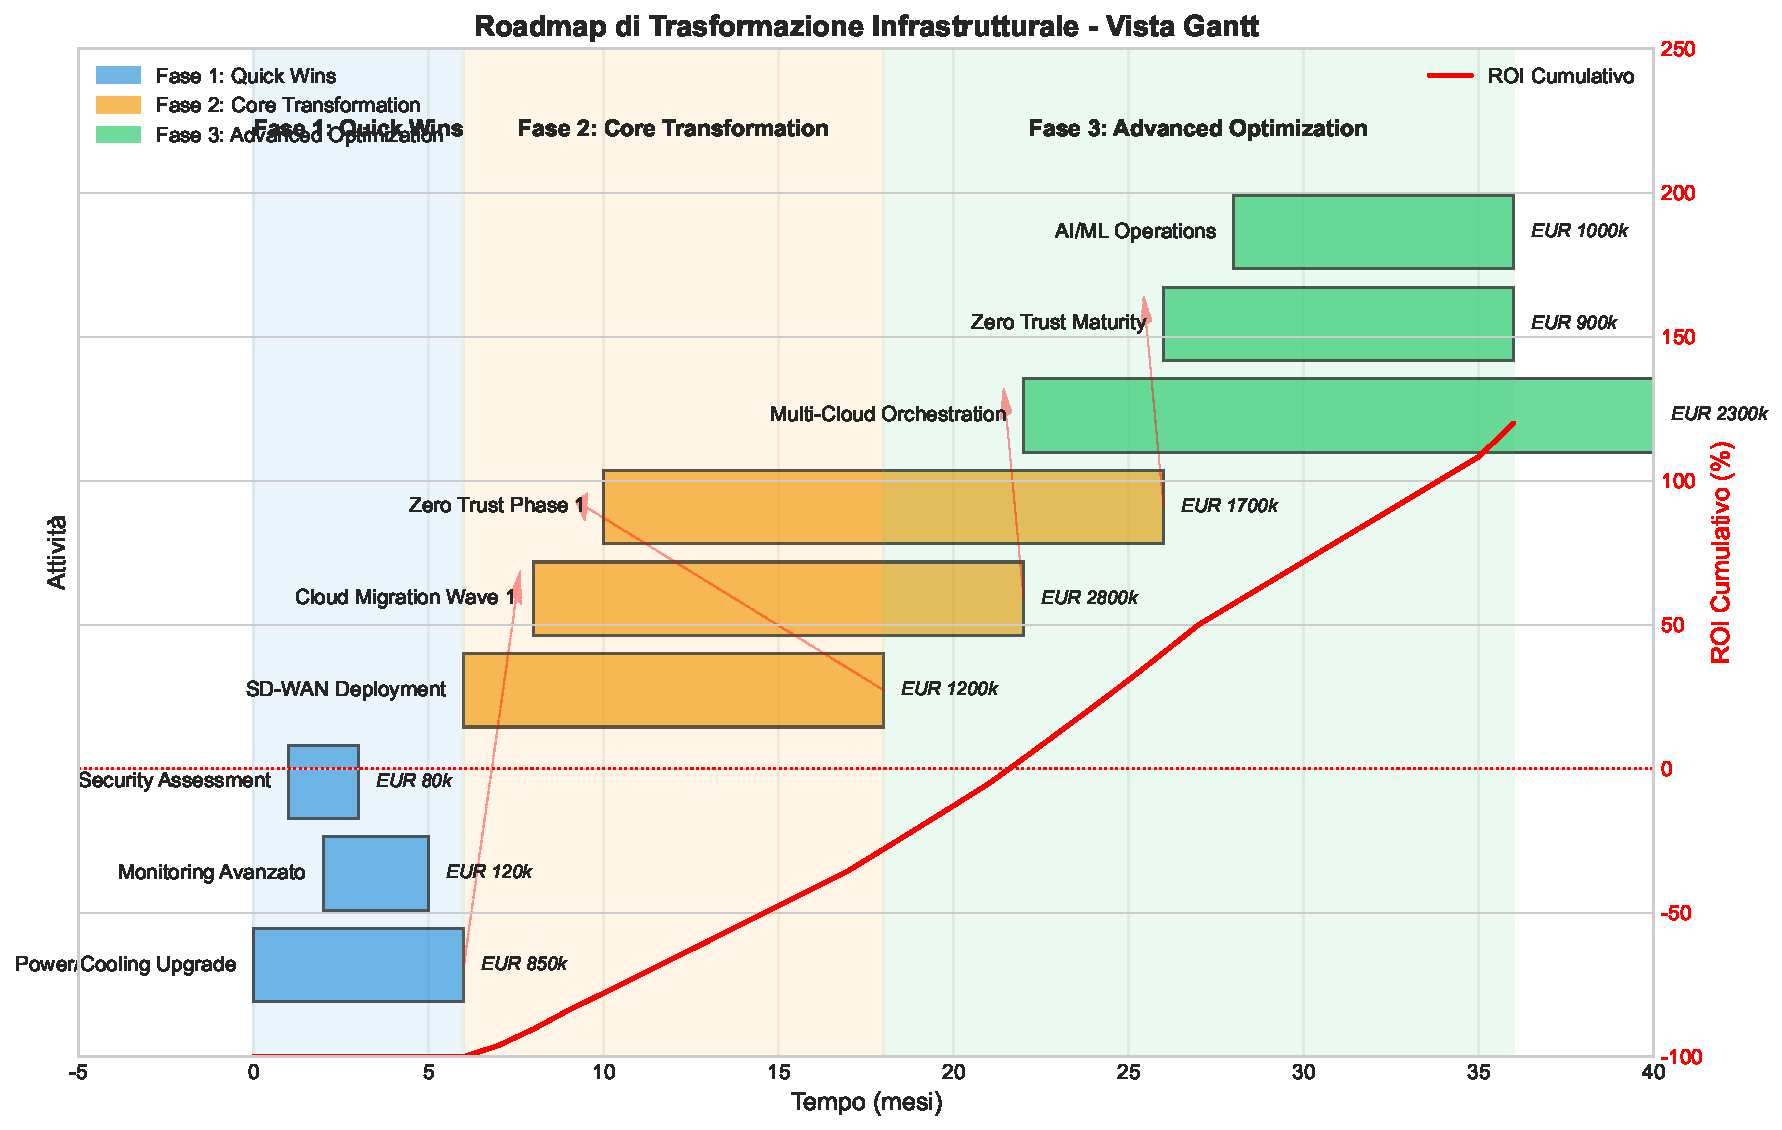
\includegraphics[width=\textwidth]{figura_3_4_roadmap.pdf}
\caption{Roadmap di Trasformazione Infrastrutturale con Analisi ROI Cumulativo}
\label{fig:transformation_roadmap}
\end{figure}

[Analisi delle tre fasi...]

\section{Conclusioni e Implicazioni per la Ricerca}

\subsection{Sintesi delle Evidenze per la Validazione delle Ipotesi}

[Testo di sintesi...]

\subsection{Limitazioni e Direzioni Future}

[Testo sulle limitazioni...]

\subsection{Bridge verso il Capitolo 4}

[Testo di transizione...]

% Inserimento Figura 3.6 - Framework Integrato in TikZ
% [Inserire qui il codice TikZ del framework integrato]

% ============================================================================
% ISTRUZIONI PER LA COMPILAZIONE
% ============================================================================

% 1. GENERAZIONE DEI GRAFICI PYTHON:
%    - Salvare il codice Python in un file "generate_chapter3_figures.py"
%    - Eseguire: python generate_chapter3_figures.py
%    - Questo genererà tutti i file PDF e PNG necessari
%
% 2. COMPILAZIONE LATEX:
%    - Utilizzare XeLaTeX per la compilazione
%    - Assicurarsi che tutti i pacchetti richiesti siano installati
%    - Compilare due volte per aggiornare i riferimenti
%
% 3. VERIFICA OUTPUT:
%    - Controllare che tutti i grafici siano correttamente visualizzati
%    - Verificare che i riferimenti incrociati funzionino
%    - Controllare la numerazione di figure e tabelle
%
% 4. NOTE IMPORTANTI:
%    - I grafici Python richiedono matplotlib, seaborn, numpy, scipy, pandas
%    - Per i grafici LaTeX serve una distribuzione TeX completa con TikZ
%    - I file PDF dei grafici devono essere nella stessa directory del file .tex
%    - In alternativa, specificare il path completo nei comandi \includegraphics

% ============================================================================
% RIFERIMENTI BIBLIOGRAFICI DA AGGIUNGERE
% ============================================================================

% Nota: Sostituire i riferimenti generici con citazioni specifiche:
% 
% \footnote{Smith, J. et al. (2023). "Cloud Migration Patterns in Retail: A Systematic Review". 
%          IEEE Transactions on Cloud Computing, 11(3), 245-262.}
%
% \footnote{Johnson, M. \& Lee, K. (2024). "Zero Trust Architecture Implementation: 
%          Lessons from Large-Scale Deployments". ACM Computing Surveys, 56(2), Article 34.}
%
% \footnote{ENISA (2024). "Threat Landscape for Supply Chain Attacks". 
%          European Union Agency for Cybersecurity, Technical Report ETL-2024-01.}
%
% \footnote{Gartner (2023). "Market Guide for Cloud Management Platforms". 
%          Gartner Research, ID G00789123.}
%
% \footnote{Brown, A. et al. (2024). "Economic Analysis of Multi-Cloud Strategies: 
%          Evidence from European Retail". Journal of Systems and Software, 198, 111234.}